\appendix
\onecolumn
\section{Appendix}\label{sec:appendix}
\subsection{Weighted Chord Symbol Recall}\label{app:weighted_chord_symbol_recall}

A formal definition of WCSR is provided in Equation~\ref{eq:wcsr}. The WCSR is a measure of the percentage of time that the model's predictions are correct.

\begin{equation}\label{eq:wcsr}
    WCSR = 100\cdot\frac{1}{Z}\sum_{i=1}^{N} \int_{t=0}^{T_i} M(y_{i,t},\hat{y}_{i,t}) dt
\end{equation}
\begin{equation}
    Z = \sum_{i=1}^{N} \int_{t=0}^{T_i} \mathbb{I}_M(y_{i,t}) dt
\end{equation}

where $M(y, \hat{y})\in\{0,1\}$ is the measure of correctness which varies across metrics. For example, $M(y, \hat{y})$ for \texttt{root} equals $1$ if $y$ and $\hat{y}$ share the same root and $0$ otherwise. $N$ is the number of songs, $T_i$ is the length of song $i$, $y_{i,t}$ is the true chord at time $t$ of song $i$, and $\hat{y}_{i,t}$ is the predicted chord at time $t$ of song $i$. $Z$ normalises by the length of time for which the metric $M$ is defined. This is necessary as \texttt{X} symbols are ignored and \texttt{seventh} ignores some qualities. Further details can be found in the \texttt{mir\_eval} documentation. $\mathbb{I}_M(y_{i,t})=1$ if $M$ is defined for label $y_{i,t}$ and $0$ otherwise. Finally, we multiply by 100 to convert to a percentage.

We also define WCSR for a single class $c$ in Equation~\ref{eq:wcsr_c}. This is useful for understanding the performance of the model on a specific chord class.

\begin{equation}\label{eq:wcsr_c}
    \text{WCSR}(c) = \frac{1}{Z_c}\sum_{i=1}^{N} \int_{t=0}^{T_i} M(y_{i,t},\hat{y}_{i,t}) \cdot \mathbb{I}_c(y_{i,t}) dt
\end{equation}
\begin{equation}
    Z_c = \sum_{i=1}^{N} \int_{t=0}^{T_i} \mathbb{I}_M(y_{i,t})\cdot \mathbb{I}_c(y_{i,t}) dt
\end{equation}

where $N$, $T$, $M$, $y_{i,t}$, $\hat{y}_{i,t}$ and $\mathbb{I}_M(y_{i,t})$ are defined as before in Equation~\ref{eq:wcsr}. $\mathbb{I}_c(y_{i,t})$ is $1$ if the true chord at time $t$ of song $i$ is class $c$ abd $0$ otherwise. $Z_c$ normalises by the length of time for which the chord $c$ is playing and for which the metric $M$ is defined, in a similar fashion to $Z$ in Equation~\ref{eq:wcsr}.


\subsection{Learning Rate and Scheduler Results}\label{app:learning_rate_scheduler}

Figure~\ref{fig:lr_search_cosine} shows the effect of different learning rates on training dynamics under a cosine scheduler for the \emph{CRNN}. The learning rate of $10^{-3}$ achieves the most stable convergence and highest validation performance, with diminishing returns observed beyond approximately 100 epochs. Both higher and lower learning rates lead to suboptimal optimisation behaviour, either through instability or slow convergence.

Table~\ref{tab:crnn_lr} summarises performance across learning rates and scheduling strategies. The results indicate that $10^{-3}$ consistently performs best across metrics, with only marginal differences between cosine, plateau, and no scheduling. This suggests that scheduler choice has limited impact compared to the choice of learning rate itself, and that performance is largely robust once the model is trained at an appropriate scale.

\begin{figure*}[h]
    \centering
    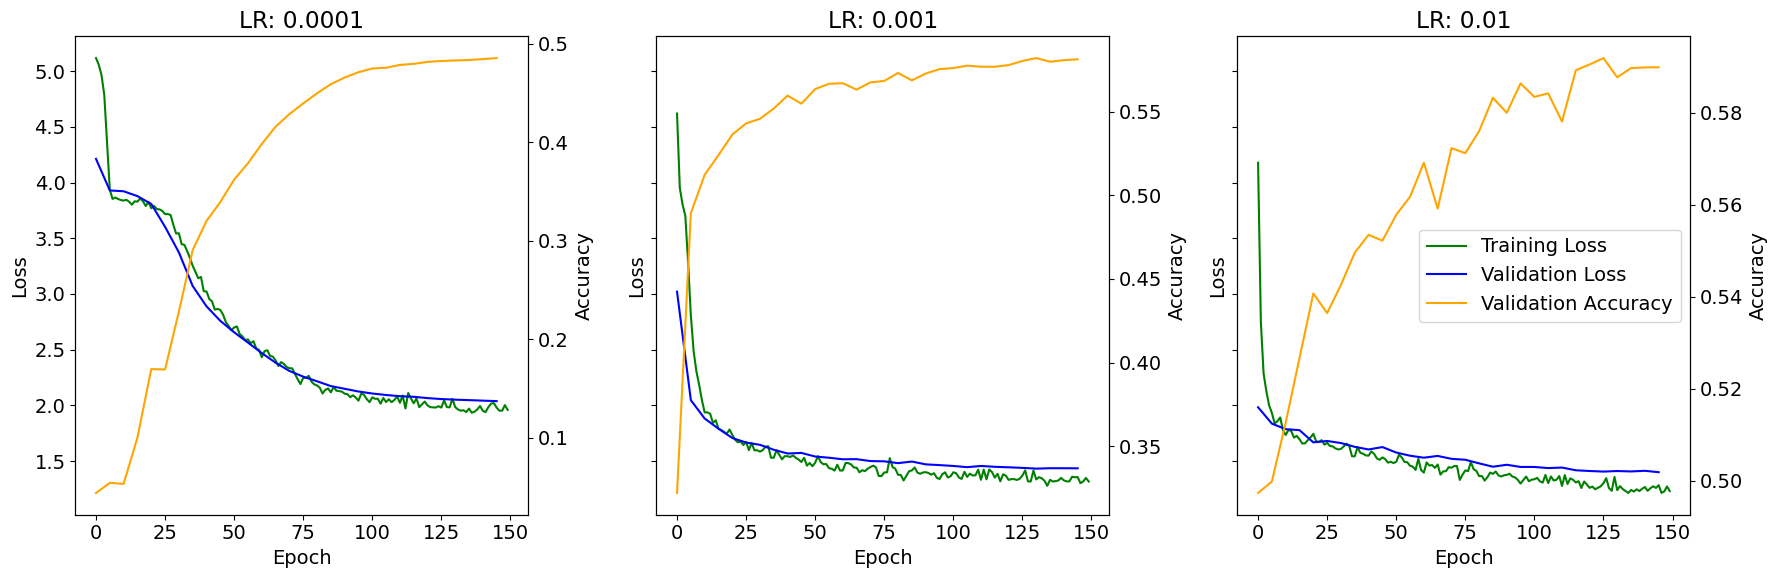
\includegraphics[width=1.0\textwidth]{figures/lr_search_cosine.png}
    \caption{Training graphs for the \emph{CRNN} with different learning rates and the \texttt{cosine} scheduler. The learning rate of $0.001$ seems to be the best, as it converges in a reasonable time and the validation accuracy increases in a stable fashion. While it may seem that running for more epochs may increase performance, this was not found to be the case empirically. The best model was often achieved around epoch 100.}\label{fig:lr_search_cosine}
\end{figure*}

\begin{table*}[h]
    \centering
    \begin{tabular}{lcccccc}
        \toprule
        lr & scheduler & acc & root & third & seventh & mirex \\
        \midrule
        0.01 & Cosine &  53.6 & 69.5 & 66.9 & 55.7 & 78.6 \\
        0.001 & Cosine & \emph{59.7} & \emph{78.3} & \emph{75.0} & \emph{62.0} & \emph{\textbf{79.8}} \\
        0.0001 & Cosine & 53.2 & 72.1 & 66.9 & 55.2 & 72.0 \\
        \midrule
        0.001 & Plateau & \textbf{59.9} & 78.4 & 75.2 & \textbf{62.2} & 79.7 \\
        0.001 & None & 59.8 & \textbf{78.7} &\textbf{75.5} & 62.0 & 78.8 \\
        \bottomrule
    \end{tabular}
    \caption{\emph{CRNN} model results with different learning rates and schedulers. Best results over learning rates are \emph{italicised} and best results over schedulers are in \textbf{boldface}. A learning rate of $0.001$ performs the best on all metrics. The differences between learning rate schedulers are so small that the choice between them is arbitrary. }\label{tab:crnn_lr}
\end{table*}


\subsection{Ablation on CRNN Model/Training}\label{app:crnn_ablation}

Using the best learning rate and learning rate scheduler from~\ref{app:learning_rate_scheduler}, we perform a random search over the number of layers in the GRU, the hidden size of the layers in the GRU the training patch segment length, the number of convolutional layers before the GRU, the kernel size of these layers and the number of channels outputted by each of these layers. The search is performed by independently and uniformly randomly sampling 50 points over discrete sets of possible hyperparameter values. 

Table~\ref{tab:crnn_hparams} shows a sample of the results. Results across hyperparameters are relatively stable. In general, increasing model complexity hurts performance and the differences between models are relatively small. Such small differences indicate that the model is learning something simple where increased model complexity does not help. It also seems that the choice of hyperparameters is somewhat arbitrary. The models do not utilise information from a larger context. Deeper layers with more parameters do not help performance. In fact, the parameters suggested by~\cite{StructuredTraining} perform just as well as the best-performing hyperparameter selection found in this random search. We therefore proceed with the same hyperparameters suggested by~\cite{StructuredTraining} as default for the remainder of experiments.

\begin{table*}[h]
    \centering
    \begin{tabular}{ccccccccccc}
        \toprule
        $L$ & $h$ & $k$ & $c$ & $g$ & $ch$ & acc & root & third & seventh & mirex \\
        \midrule
        23 & 231 & 5 & 1 & 1 & 1 & \textbf{59.8} & 78.2 & 74.7 & \textbf{62.0} & \textbf{79.9} \\
        11 & 150 & 7 & 2 & 1 & 3 & 59.6 & 78.5 & 75.0 & 61.9 & 79.2 \\
        43 & 222 & 11 & 2 & 2 & 2 & 59.5 & \textbf{78.7} & \textbf{75.2} & 61.8 & 78.9 \\
        \ldots & \ldots & \ldots & \ldots & \ldots & \ldots & \ldots & \ldots & \ldots & \ldots & \ldots \\
        34 & 159 & 14 & 4 & 2 & 1 & 56.9 & 75.5 & 72.2 & 59.1 & 77.7 \\
        \bottomrule
    \end{tabular}
    \caption{A subset of \emph{CRNN} model results on the large vocabulary with different hyperparameters. The best results for each metric are in boldface. $L$ is the length of training patches of audio in seconds, $h$ and $g$ are the hidden size and number of layers in the GRU respectively and $k$, $c$ and $ch$ are the kernel sizes, number of layers and number of channels in the CNN respectively. Models are ordered by their `Rank', calculated by adding the model's rank order over each metric and ordering by this total. Results across most hyperparameters are very similar. Comparing with the best results from the learning rate search in Table~\ref{tab:crnn_lr}, it seems that the parameters suggested by \cite{StructuredTraining} are good choices. Models with more parameters and longer input tend to perform worse, perhaps due to overfitting. This suggests that the model is learning something simple.}\label{tab:crnn_hparams}
\end{table*}

\subsection{Hop Lengths}\label{app:hop_lengths}

Different hop lengths have been used to calculate the CQT ranging from 512~\cite{ACRLargeVocab1} up to 4096~\cite{StructuredTraining}. In previous experiments we have used a hop length of $4096$ as is used by the authors of \emph{CRNN}~\cite{StructuredTraining}. Shorter frames would reduce the number of transition frames but require more computational cost. If frame lengths are too short, the Fourier transform may not be able to capture the harmonic structure of the audio.

In Table~\ref{tab:hop_lengths}, we test the effect of different hop lengths on the model's performance. We use a CQT with $216$ bins and a hop length of $512$, $1024$, $2048$, $4096$, $8192$ and $16384$. Results indicate that performance is similar for hop lengths of $4096$ and below. Performance suffers for greater hop lengths. While it could be argued that $2048$ does better than $4096$, this difference is small enough that it is not worth the increased computational cost. Models trained with a hop size of $2048$ take at least twice as long to train and evaluate as those trained on a hop size of $4096$.

\begin{table*}[h]
    \centering
    \begin{tabular}{lccccc}
        \toprule
        hop length & acc & root & third & seventh & mirex \\  
        \midrule
        512 & 60.1 & 78.3 & \textbf{75.5} & 62.4 & \textbf{80.0} \\
        1024 & 60.2 & \textbf{78.7} & 75.2 & 62.5 & 79.6 \\
        2048 & \textbf{60.3} & 78.5 & 75.2 & \textbf{62.6} & 79.6 \\
        4096 & 60.0 & 78.1 & 75.0 & 62.2 & 79.2 \\
        8192 & 57.9 & 76.2 & 72.9 & 60.1 & 79.3 \\
        16384 & 53.3 & 71.7 & 68.0 & 55.4 & 77.9 \\
        \bottomrule
    \end{tabular}
    \caption{Results over different hop lengths for CQT calculation. Any hop length in the range $512$ to $4096$ has similar performance. For frames that are any longer, performance suffers. This is likely caused by the requirement for the model to assign a single chord class to each frame. The longer the frame, the greater potential there is for multiple chords to be playing during the frame. }\label{tab:hop_lengths}
\end{table*}

\subsection{Output Smoothing}\label{app:output_smoothing}

The \emph{CRNN} with no smoothing predicts an average of $168$ transitions per song as opposed to the $104$ seen in the ground truth data. We implement a decoding step over the frame-wise probability vectors to smooth predicted labels. Common choices for decoding models include a conditional random field (CRF)~\cite{ACRLargeVocab1, BTC} and a hidden Markov model (HMM)~\cite{BalanceRandomForestACR}. 

We first implement a HMM. The HMM treats the frame-wise probabilities as emission probabilities and the chord labels as hidden states. \cite{CQTvsChroma} note that using a transition matrix with homogeneous off-diagonal entries in the transition matrix performs similarly to using a learned transition matrix. We adopt such a transition matrix for this HMM, with a parameter $\beta$ denoting the probability of self-transition and all other transition probabilities equal to $\frac{1-\beta}{C-1}$. Decoding then follows the Viterbi algorithm~\cite{Viterbi} over the summed forward and backward pass.

A plot of the effect of $\beta$ on the model's performance and the number of transitions per song is shown in Figure~\ref{fig:hmm_beta_search}. From this plot, we conclude that smoothing has little effect on the performance of the model while successfully reducing the number of transitions per song to that of the true labels. We select $\beta = 0.15$ for the remainder of experiments as it results in $102$ transitions per song while maintaining high performance. 

\begin{figure*}[ht]
    \centering
    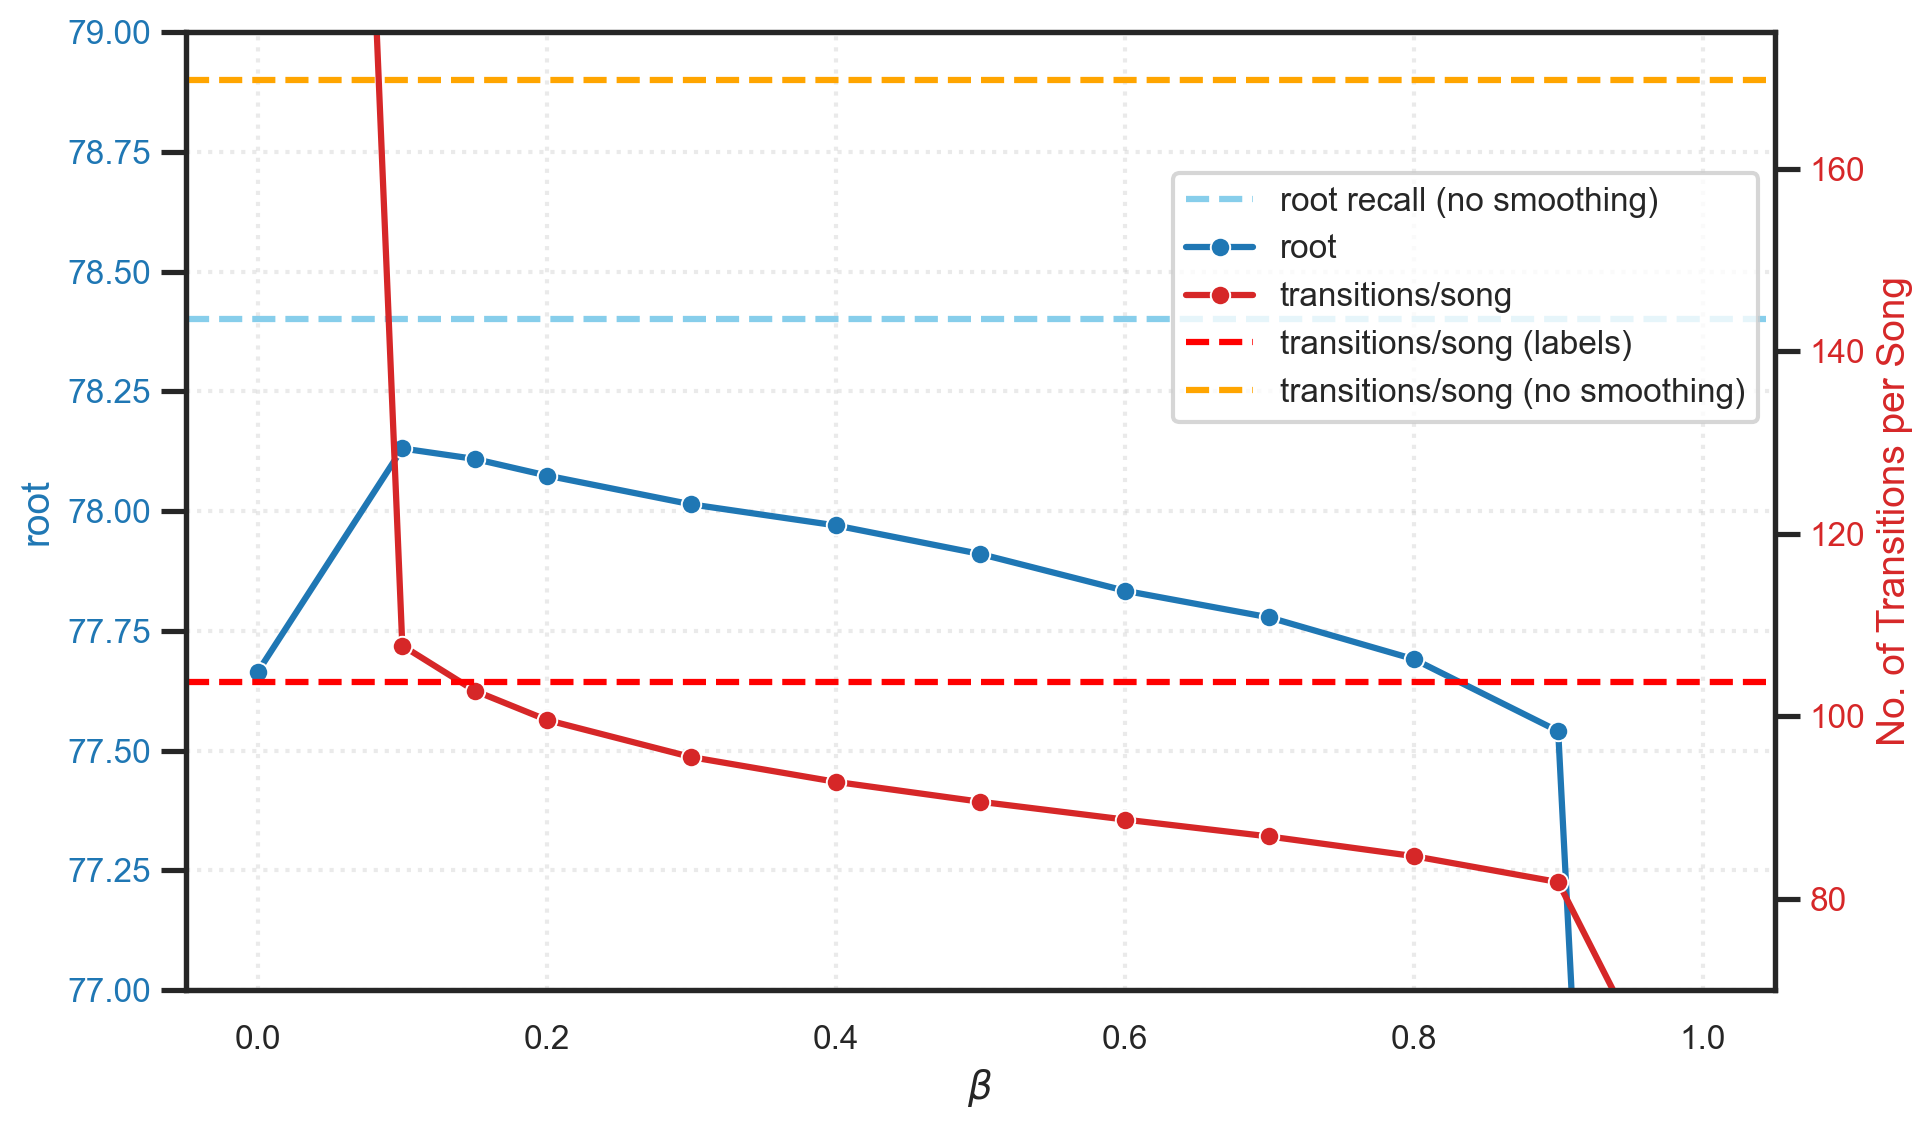
\includegraphics[width=0.8\textwidth]{figures/hmm_beta_vs_root_transitions.png}
    \caption{Effect of the HMM smoothing parameter $\beta$ on the \emph{CRNN} model. As we increase $\beta$, the number of transitions per song decreases. We choose $\beta = 0.15$ as it results in $102$ transitions per song, very close to the $104$ of the ground truth. Performance is stable across $\beta$ with a slight degradation for $\beta > 0.3$. Other performance metrics showed similarly stable results. }\label{fig:hmm_beta_search}
\end{figure*}

We also implement a linear chain CRF using \texttt{pytorch-crf}.\footnote{\url{https://github.com/kmkurn/pytorch-crf}} In contrast to the HMM, the CRF uses a learned transition matrix. Results comparing the HMM, CRF and no smoothing can be found in Table~\ref{tab:smoothers}. Both the CRF and HMM reduce the number of transitions per song to a similar level. The HMM outperforms the CRF with $3.5\%$ greater accuracy. The HMM has almost identical performance to the model with no smoothing. We hypothesise that the learned transition matrix allows the model to overfit to the chord sequences in the training set. Regardless of the explanation, we proceed with HMM smoothing.

\begin{table*}[h]
    \centering
    \begin{tabular}{lcccccc}
        \toprule
        smoother & acc & root & third & seventh & mirex & transitions/song\\  
        \midrule
        none & \textbf{60.0} & \textbf{78.1} & \textbf{75.0} & \textbf{62.3} & \textbf{79.2} & 167 \\
        HMM & \textbf{60.0} &\textbf{78.1} & \textbf{75.0} & \textbf{62.3} & \textbf{79.2} & \textbf{102} \\
        CRF & 56.5 & 75.5 & 72.5 & 58.6 & 76.2 & 100 \\
        \bottomrule
    \end{tabular}
    \caption{Results for the HMM and CRF smoothing methods with the \emph{CRNN}. The HMM has almost identical performance to the model with no smoothing. Smoothing must correct predictions for roughly the same amount of time as it introduces errors. However, it drastically reduces the number of transitions per song to an acceptable level. The CRF performs notably worse than the HMM. }\label{tab:smoothers}
\end{table*}

\subsection{Pitch Augmentation}~\label{app:pitch_augmentation}

Pitch augmentation can be done directly on the CQT~\cite{ACRLargeVocab1} or on the audio~\cite{BTC,StructuredTraining}. Although similar, these are not identical transformations as shifting the CQT takes place after discarding phase information and leaves empty bins behind, whereas audio pitch shifting can introduce other artefacts intended to preserve harmonic structure and maintain phase information.

When a sample is drawn from the training set, it is shifted with probability $p$. The shift is measured in semitones in the set $\{-5,-4\ldots -1, 1, \ldots 6\}$ with equal probability of each shift. This results in 12 times as much training data. Convergence is still reached in 150 epochs. Shifting the CQT matrix is done by moving all items up or down by the number of bins corresponding to the number of semitones in the shift. 

The remaining bins are filled with a value of -80dB. Audio shifting is done with \texttt{pyrubberband}.\footnote{\url{https://github.com/bmcfee/pyrubberband}}. CQTs are then calculated on the shifted audio. A plot of the effect of the shift probability $p$ on the model's performance can be found in Figure~\ref{fig:pitch_augmentation}.

Results show a clear trend that increasing $p$ improves performance. Shifting the audio provides a very similar effect to simply shifting the CQT. Choosing $p=0.9$ results in a $2.1\%$ increase in accuracy. The \texttt{mirex} score breaks the trend with performance varying over different values for $p$. The acc\textsubscript{class} metric also improves by more than $2\%$. This can be explained by the model becoming becoming root-invariant. With $p=0.9$, all potential roots become close to equally likely. We proceed with pitching shifting with $p=0.9$ on the CQT for the remainder of the experiments as it is computationally cheaper than shifting the audio.

Note that the weights for the weighted loss are calculated based on \emph{expected} counts, taking into account the shift probability $p$. We also test shifting on both the CQT and audio but the results are not different than shifting with either method alone. Unfortunately, it was not computationally feasible to test pitch shifting with generative features as the feature extraction over $12 * 1210 = 14,520$ songs is too expensive.

\begin{figure*}[h]
    \centering
    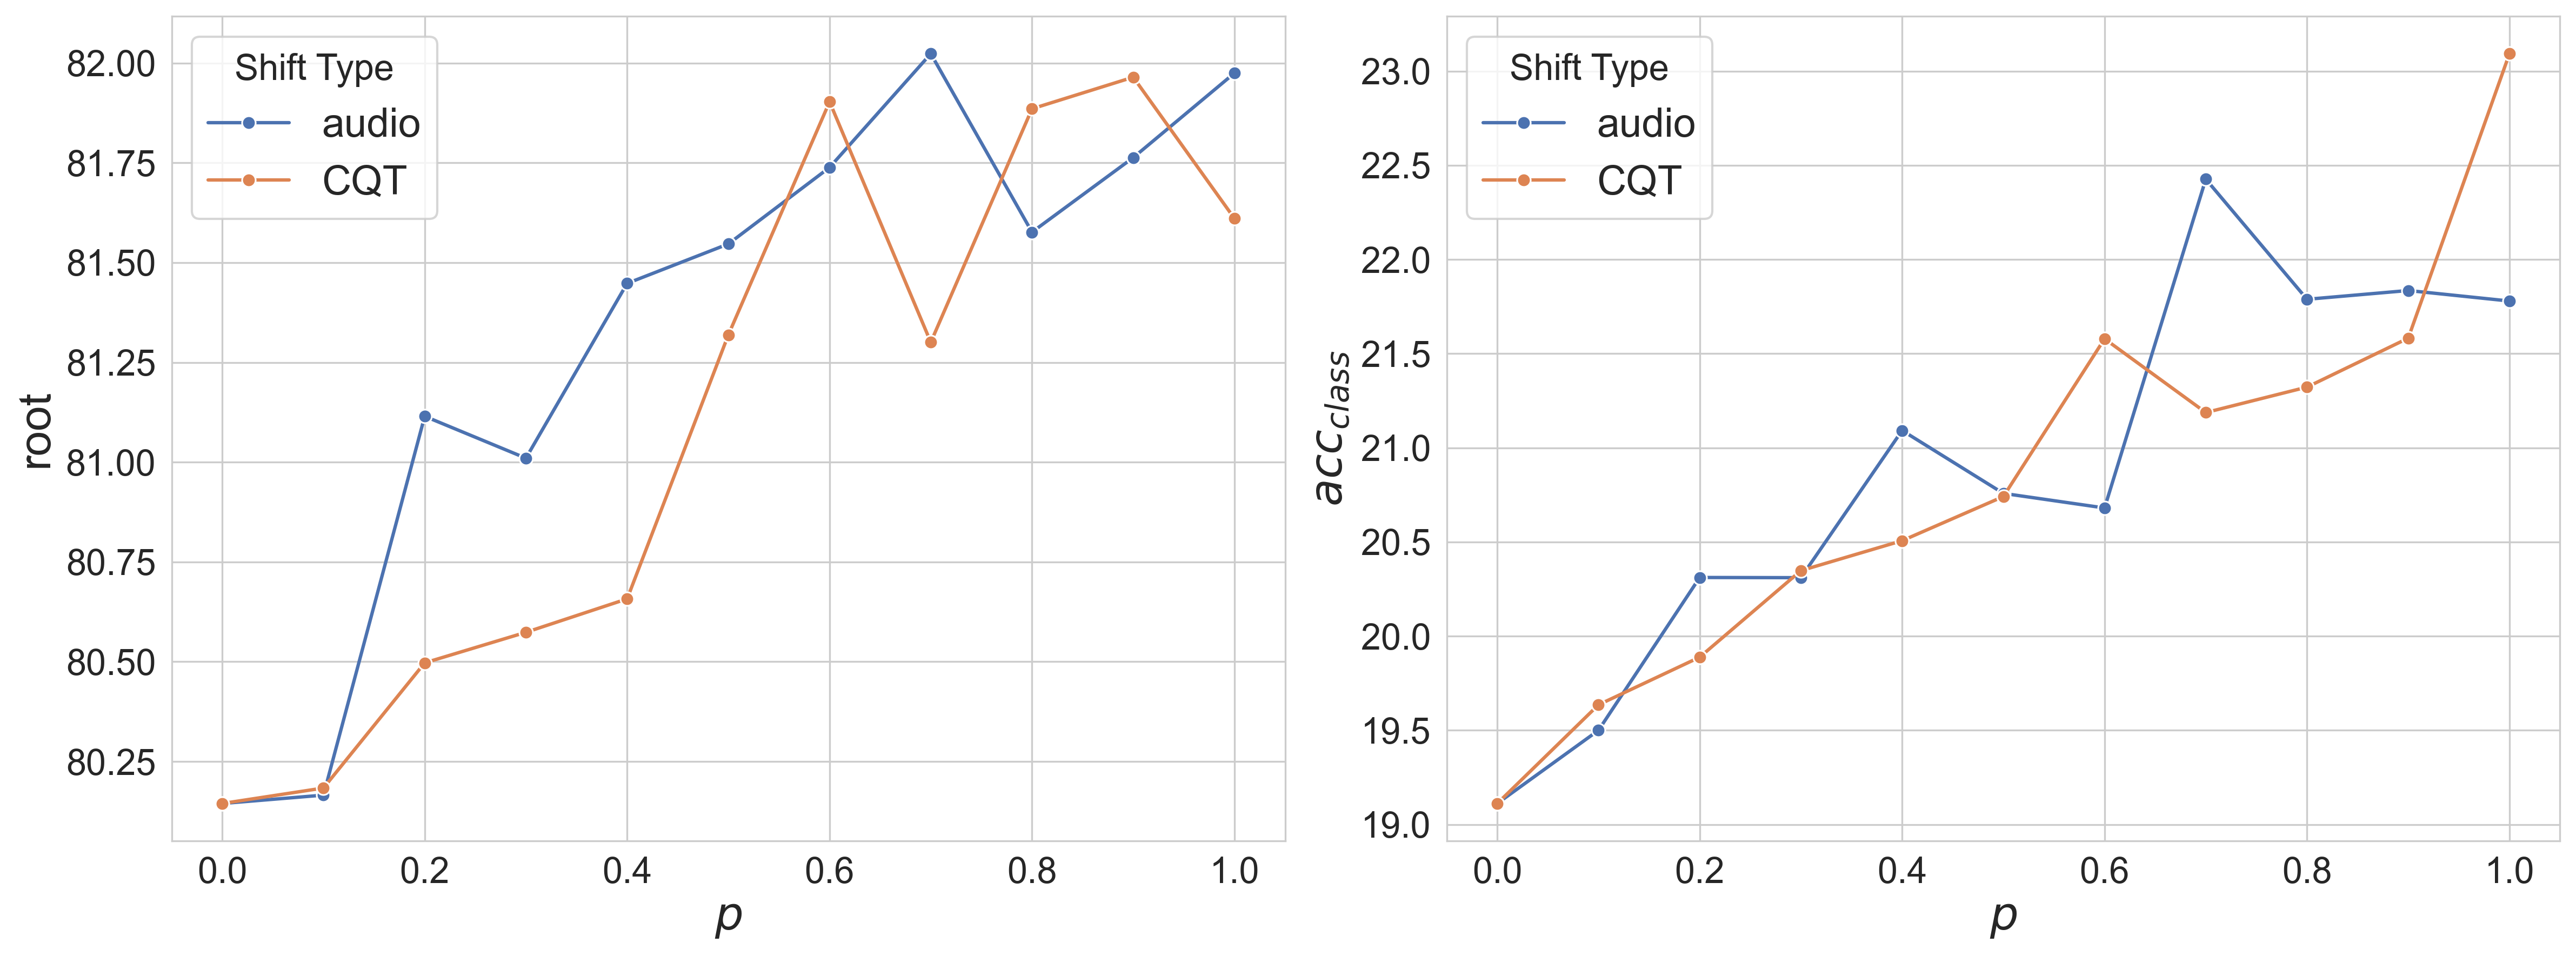
\includegraphics[width=1.0\textwidth]{figures/pitch_shift_analysis.png}
    \caption{Effect of pitch shift probability $p$ on \texttt{root} (left) and acc\textsubscript{class} (right). Pitch shifting provides a clear increase in performance. Shifting the audio or the CQT has a similar effect. We choose $p=0.9$, which is close to making the model root-invariant.}\label{fig:pitch_augmentation}
\end{figure*}


\subsection{Weighted Loss}\label{app:weighted_loss}

One of the greatest difficulties in ACR is the few instances of rare chord qualities. Two standard methods for dealing with long-tailed distributions are weighting the loss function and over-sampling. \cite{CurriculumLearning} also explore the use of curriculum learning as a form of re-sampling which we do not explore here because they report only minor performance gains. Sampling is explored by~\cite{BalanceRandomForestACR}, but they use a different model based on pre-computing chroma vectors and re-sampling these chroma vectors for use in training a random forest for frame-wise decoding. In our setting, re-sampling training patches of audio may be interesting to explore but is left as future work. It would require a complex sampling scheme as frames cannot be sampled independently. 

Weighting has been explored by~\cite{ACRLargeVocab1}. We employ a similar but simpler implementation here. A standard method of weighting is to multiply the loss function by the inverse frequency of the class of the current training sample, with a parameter controlling the strength of the weighting. This is defined in Equation~\ref{eq:weighting}.

\begin{equation}\label{eq:weighting}
    w_c = \frac{1}{{(\text{count}(c) + 10)}^\alpha}
\end{equation}

where $w_c$ is the weight for chord $c$, $\text{count}(i)$ is the number of frames with chord $c$ in the dataset and $\alpha$ is a hyperparameter controlling the strength of weighting. $\alpha=0$ results in no weighting and increasing $alpha$ increases the severity of weighting. We add $10$ in the denominator to avoid dividing by $0$ and to diminish the dominating effect of chords with very few occurrences. We then define normalised weights $w_c^*$ in Equation~\ref{eq:weighted_loss}.


\begin{equation}\label{eq:weighted_loss}
    w_c^* = \frac{w_c}{s} \text{ where } s = \frac{\sum_{c\in \mathcal{C}} \text{count}(c)\cdot w_c}{\sum_{c\in \mathcal{C}} \text{count}(c)}
\end{equation}

Where $\mathcal{C}$ is the set of all chords in the vocabulary. This keeps the expected weight over samples at $1$ such that the effective learning rate remains the same. These values are calculated over the training set. We test values of $\alpha$ in the set \{0, 0.05, 0.1, \ldots, 0.95, 1\}. The plot in Figure~\ref{fig:weighted_loss} illustrates the effect of the weighting on the model's performance. We find that increasing $\alpha$ improves \texttt{acc}\textsubscript{class} but decreases \texttt{root} accuracy. Choosing $\alpha = 0.3$ maximises \texttt{acc}\textsubscript{class} without hurting root accuracy which we carry forward to subsequent experiments.

\begin{figure*}[h]
    \centering
    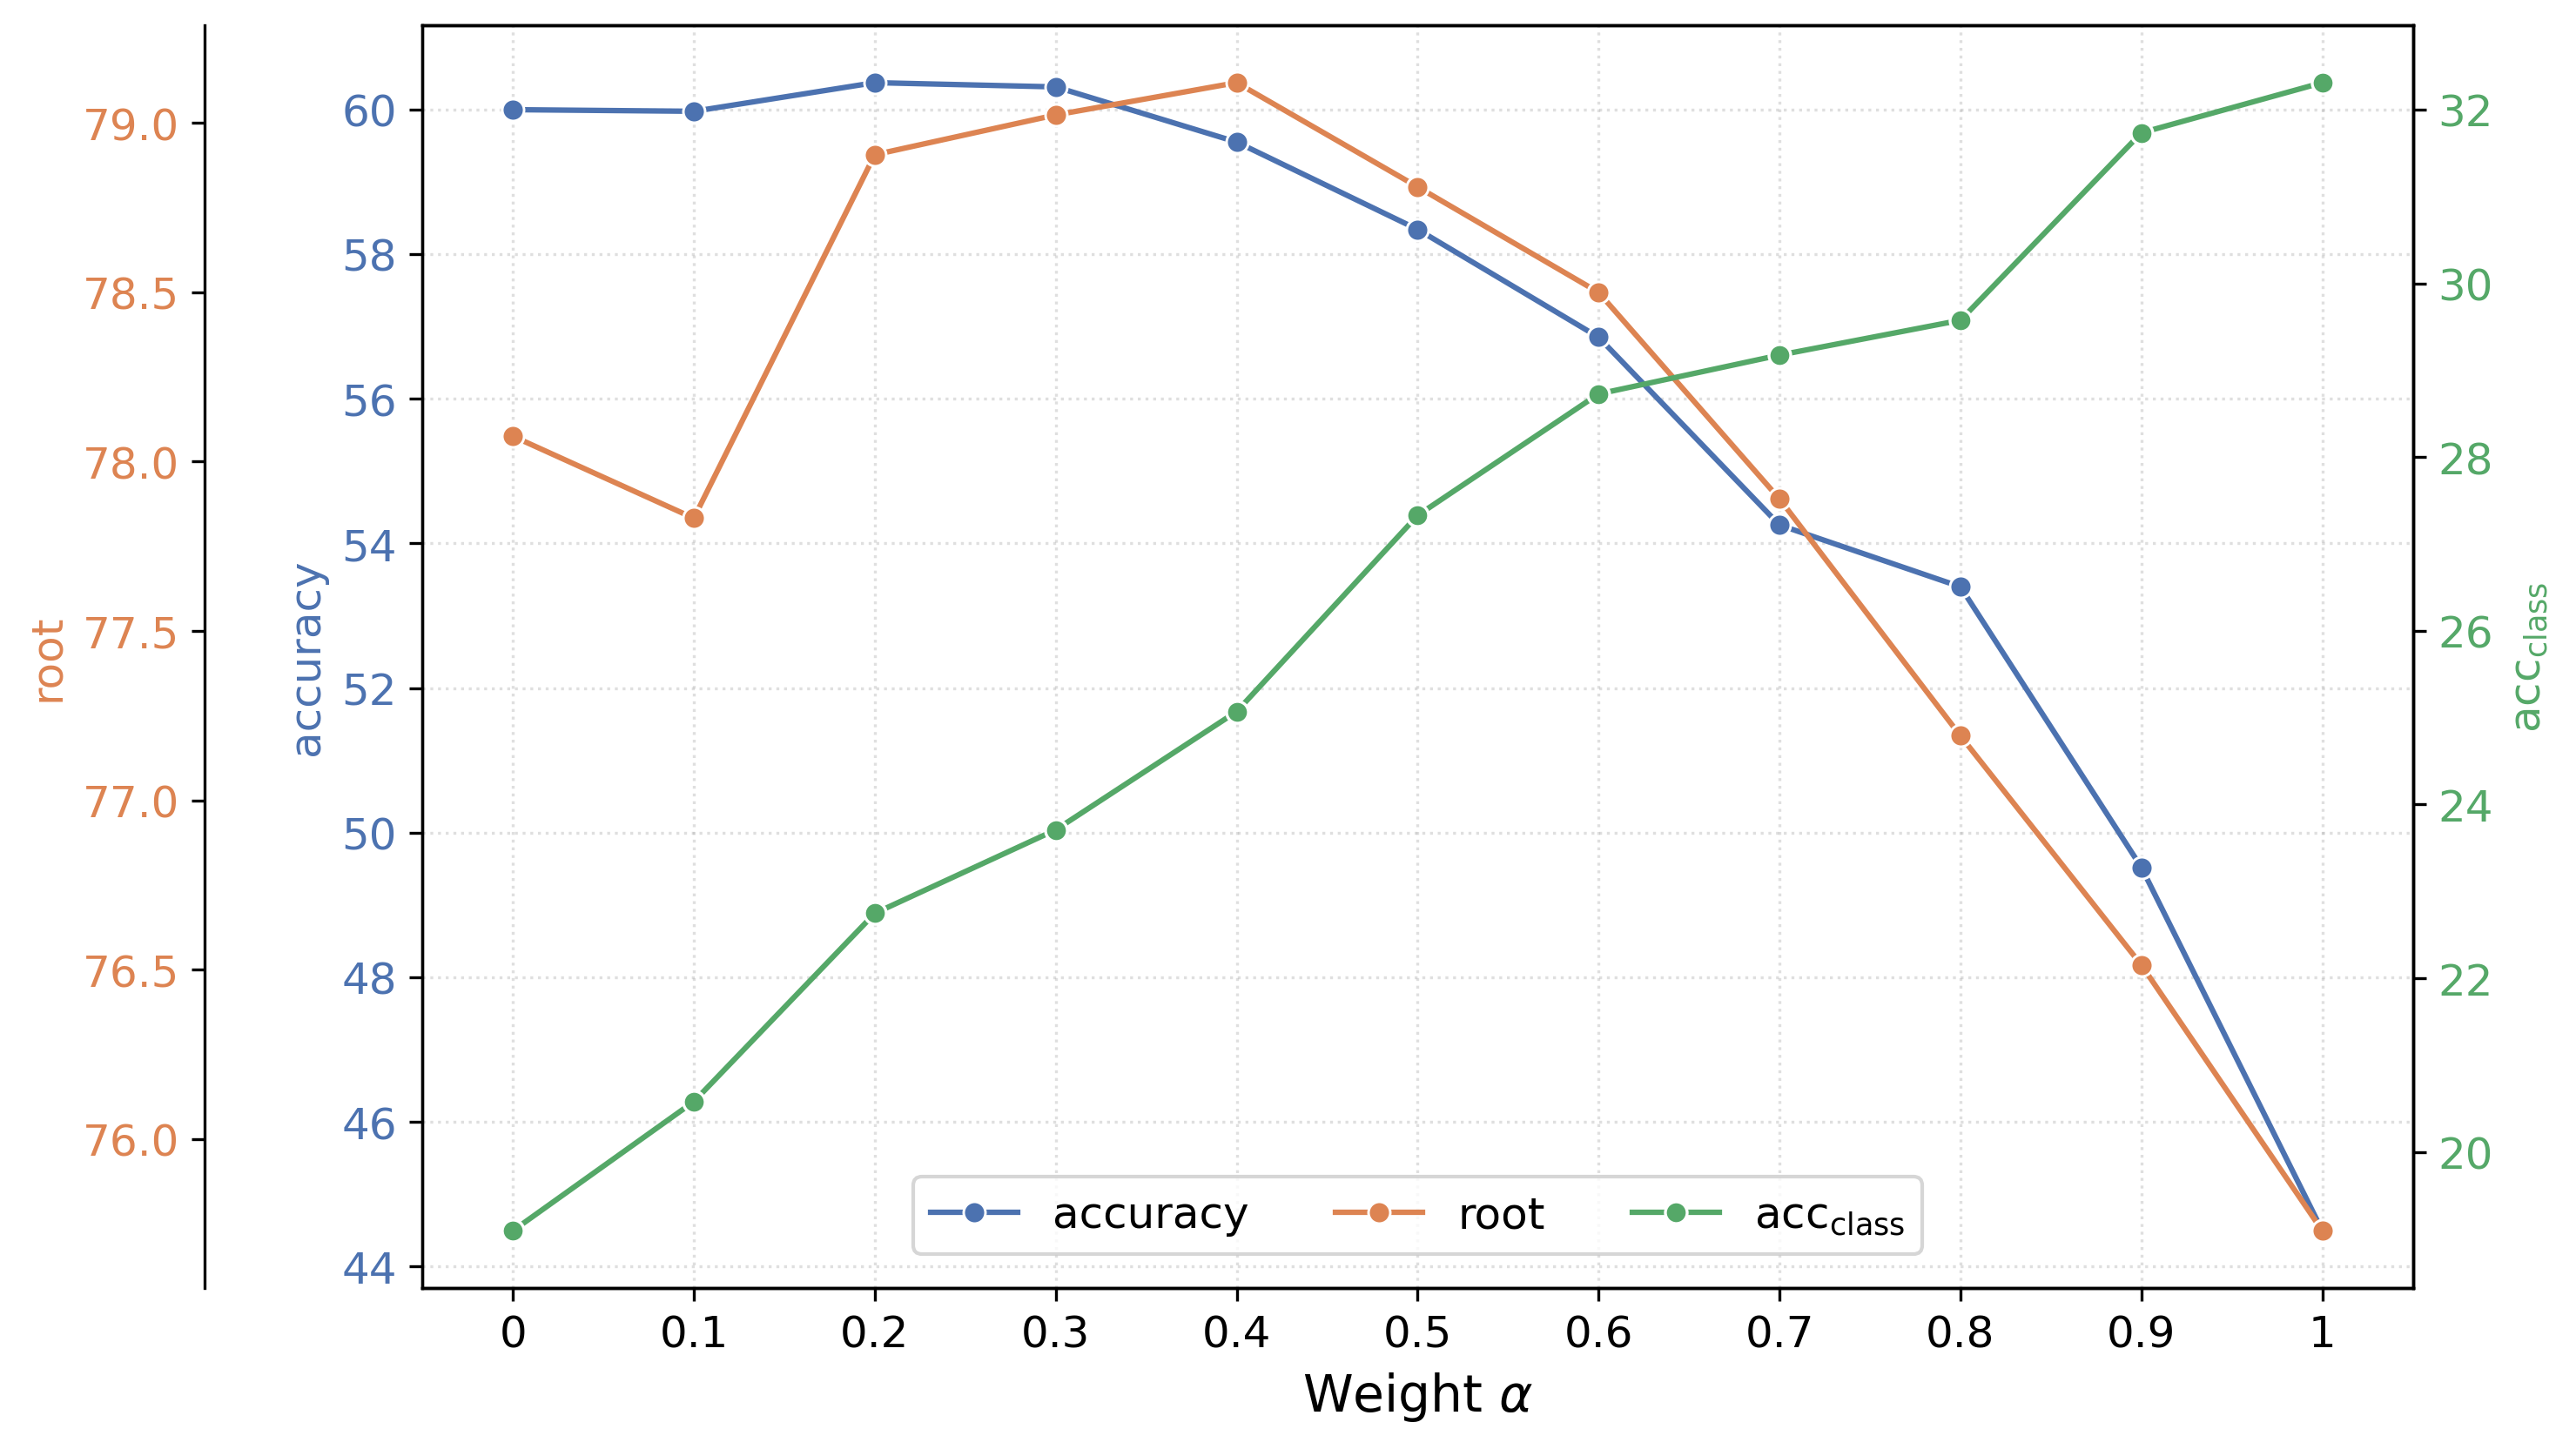
\includegraphics[width=0.8\textwidth]{figures/weight_alpha_search_trim.png}
    \caption{Effect of weighted loss on the \emph{CRNN} model with varying $\alpha$. As we increase $\alpha$, \texttt{acc}\textsubscript{class} improves accuracy and \texttt{root} decreases. We claim there is a sweet spot where very little overall performance is sacrificed for better class-wise accuracies. We select $\alpha = 0.3$. The \texttt{root} and \texttt{third} metrics improve and less than $3\%$ is lost on other metrics while mean class-wise accuracy improves by $6\%$.}\label{fig:weighted_loss}
\end{figure*}

Weighting the loss function also slightly increases the number of transitions predicted per song. This may be because occasional sharp gradient updates cause more extreme probability outputs. we increase the HMM smoothing parameter $\beta$ to $0.2$ to bring the number of transitions per song to $104$.

\subsection{Structured Loss}\label{app:structured_loss}

\cite{StructuredTraining} propose a structured loss function. They introduced additional targets for the root, bass and pitch classes. We follow a similar method but do not include the bass as the current chord vocabulary does not consider inversions. The idea behind this loss term is to explicitly task the model with identifying the components of a chord we care about. This can allow the model to exploit structure in the chord vocabulary such as shared roots and pitch classes, rather than all symbols being predicted independently.

The root can be any of the 12 notes in the Western chromatic scale, \texttt{N} or \texttt{X}, creating a 14-dimensional classification problem. The 12 pitch classes each represent a single binary classification problem. Two fully connected layers calculate a 14-dimensional vector and 12-dimensional vector from the hidden representation outputted from the GRU for the root and pitch classes, respectively. Finally, these representations are concatenated with the GRU representations and fed into the final fully connected layer to predict the chord symbol.

The mean cross-entropy loss is calculated in each case. These are summed to form the \emph{structured loss}. The final loss is a convex combination of the original loss and the structured loss as defined in Equation~\ref{eq:structured_loss}.

\begin{equation}\label{eq:structured_loss}
    L = \gamma L_{chord} + (1-\gamma)(L_{root} + L_{pitch})
\end{equation}

Where $L$ is the overall loss, $L_{chord}$ is the cross-entropy loss over chords symbols, $L_{root}$ is the cross-entropy loss targeting the root, $L_{pitch}$ is mean binary cross-entropy over each of the pitch classes. $\gamma$ is a hyperparameter controlling the weighting of the original loss. 

We test models with $\gamma\in\{0, 0.1 \ldots 0.9\}$. Choosing $\gamma=0.7$ improves accuracy by $1.3\%$ while \texttt{mirex} worsens by $0.3\%$. Accuracy with \texttt{third} increases by $1.7\%$ and on \texttt{seventh} by $1.3\%$. Generally, greater $\gamma$ improves accuracy metrics while \texttt{mirex} results are noisy. A plot of the trend can be found in Figure~\ref{fig:structured_loss}. We keep $\gamma=0.7$ from now on based on peak accuracy.

\begin{figure*}[h]
    \centering
    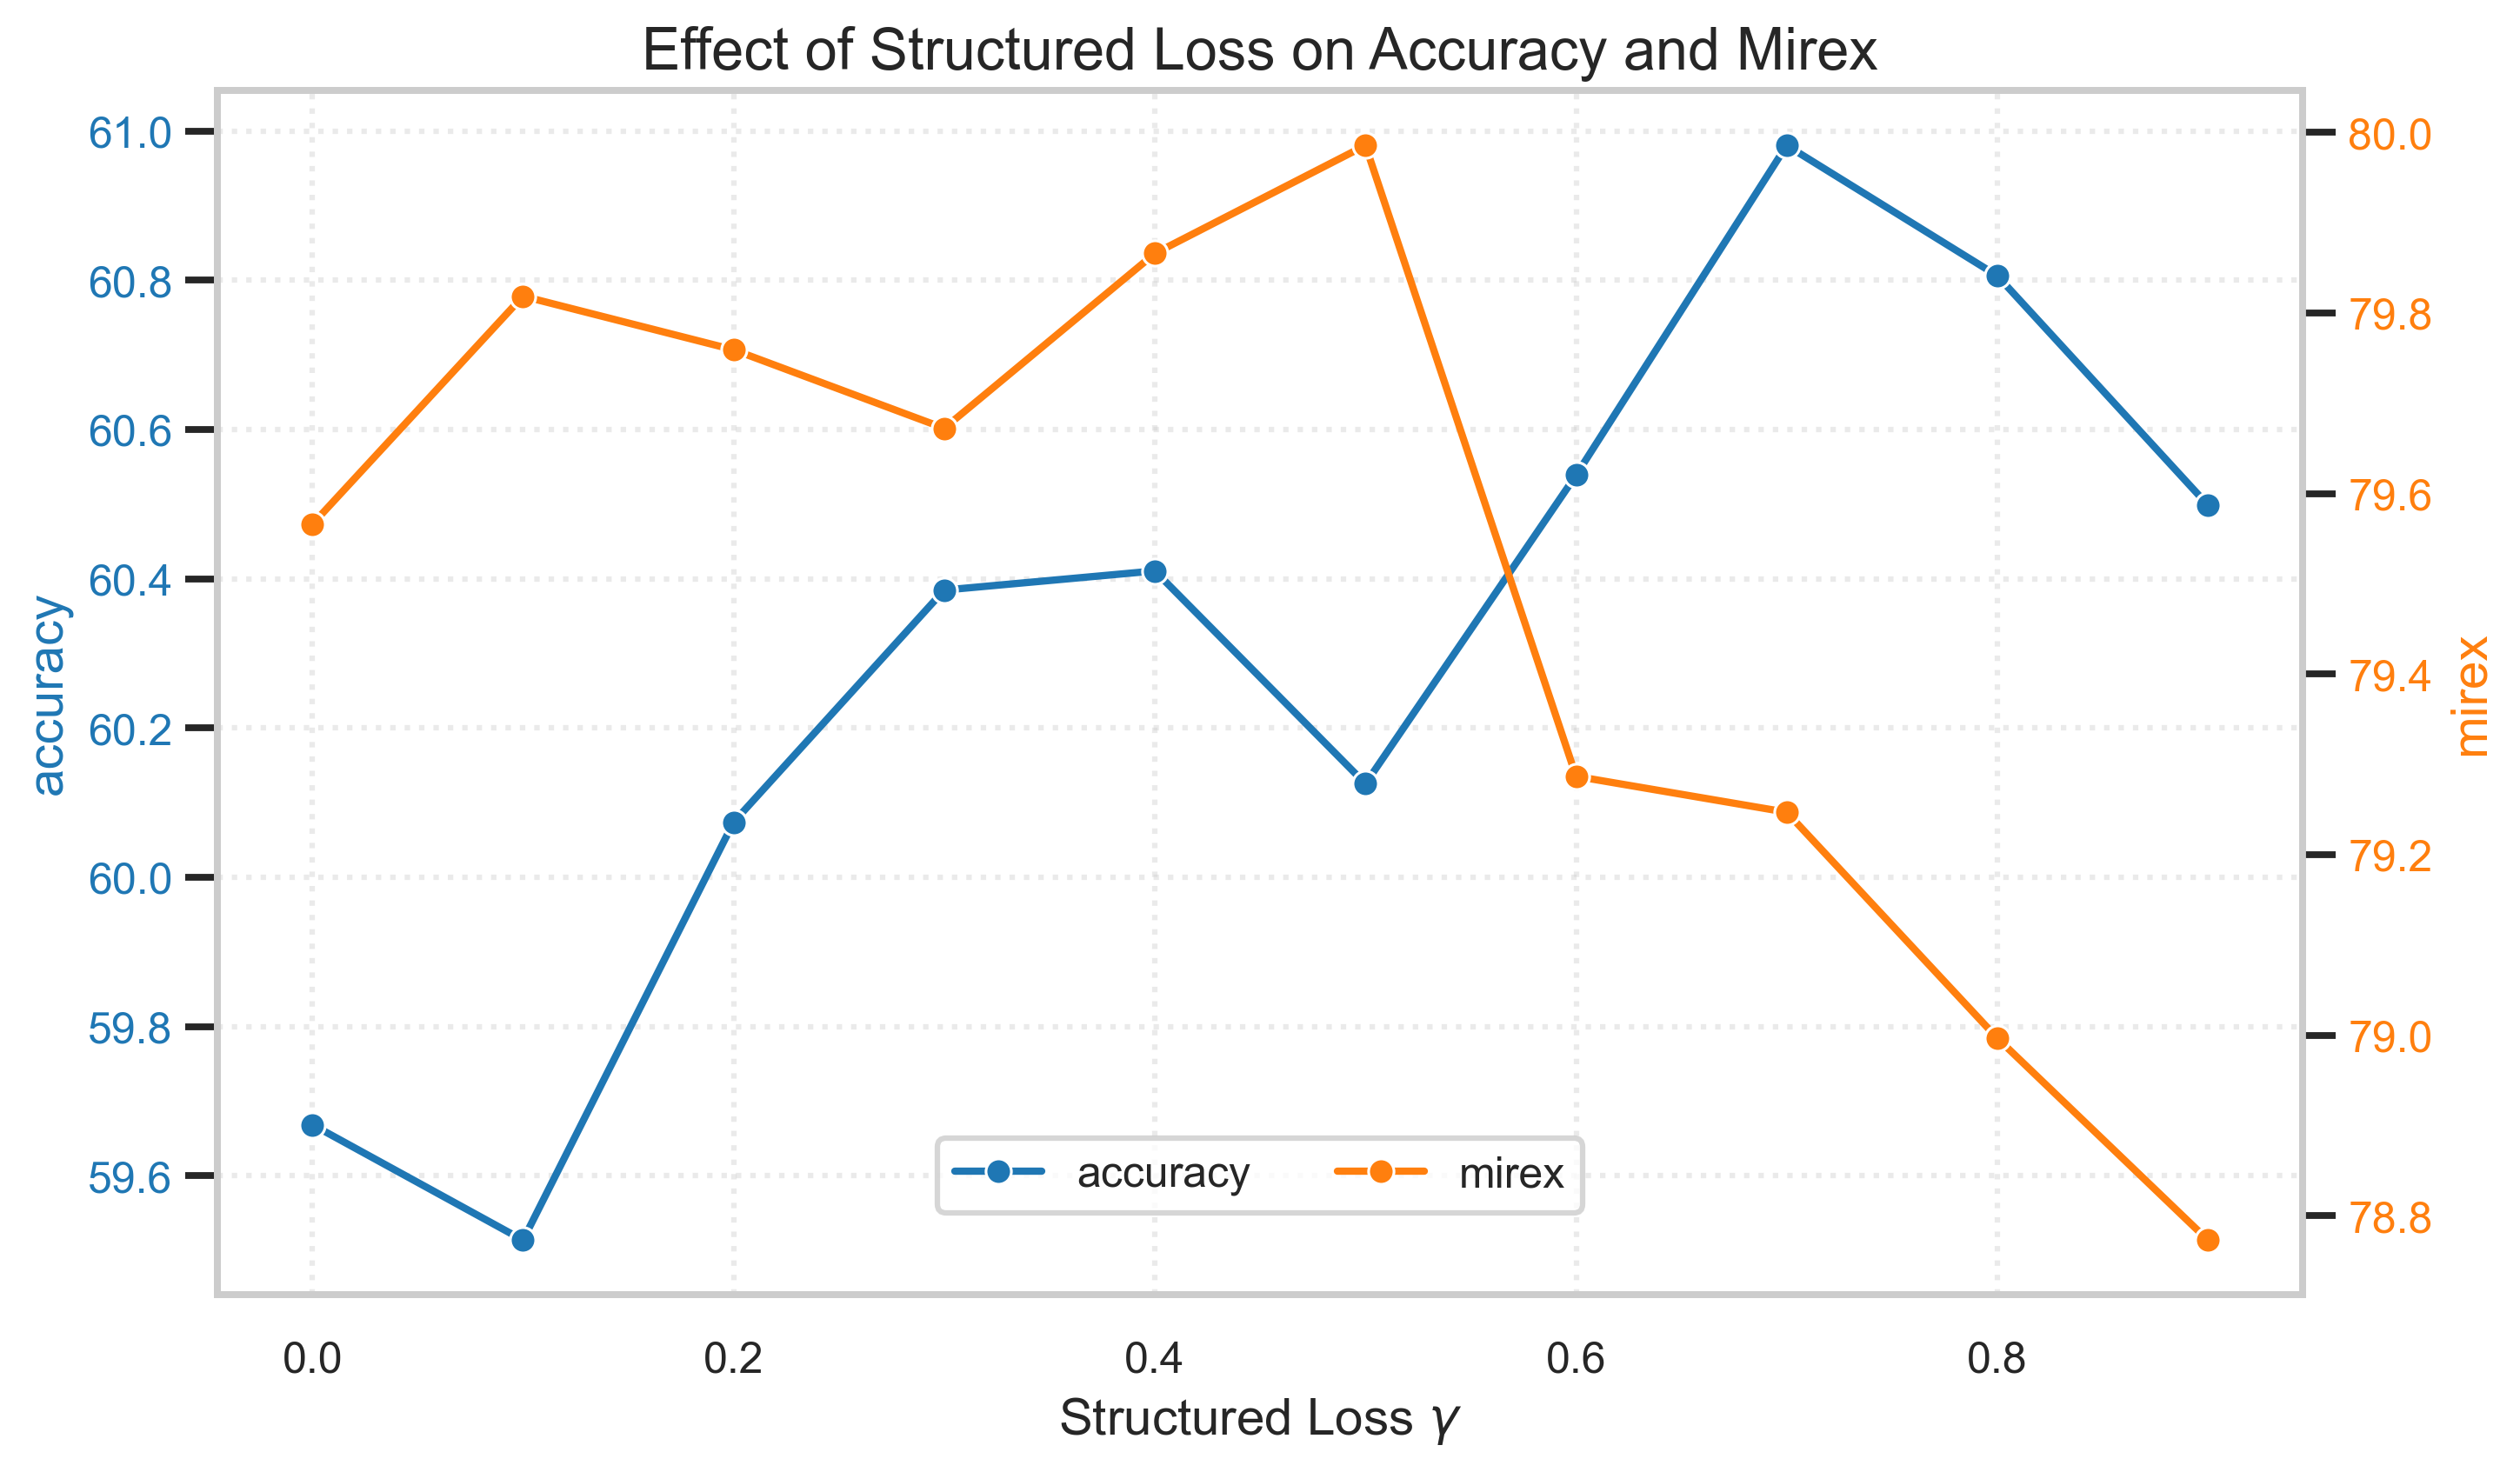
\includegraphics[width=0.8\textwidth]{figures/structured_loss_accuracy.png}
    \caption{Effect of structured loss on the \emph{CRNN} model with varying $\gamma$. As we increase $\gamma$, accuracy improves but \texttt{mirex} behaves erratically, worsening at the higher end. The other metrics behave similarly to accuracy. We choose $\gamma=0.7$ based on peak accuracy. }\label{fig:structured_loss}
\end{figure*}

\subsection{Details of Generative Feature Extraction}\label{app:generative_feature_extraction}

Overlapping $5$ second chunks of audio were fed through MusicGen in a batched fashion. This first requires passing the audio through the pre-trained Encodec audio tokeniser~\cite{Encodec}. These are then fed through the language model. We take the output logits as the representation for each frame. The model outputs logits in four `codebooks', each $2048$-dimensional vectors, intended to represent different granularities of detail in the audio. Audio segments are overlapped such that every frame has context from both directions. The multiple representations for each frame are averaged. Finally, these representations are upsampled. The model operates at a frame rate of 50Hz. To compute a representation with the same frame length as the CQT, we take the mean over the frames outputted by the model closest to the centre of the CQT frame. In case averaging over frames dampened the signal, we also tried linearly interpolating between the two closest frames outputted by the model. However, this was empirically found to perform slightly worse. Results can be found in Appendix~\ref{app:linear_interpolation_vs_area_averaging}. This feature extraction required the use of NVIDIA RTX A6000 GPUs. The extraction process took approximately 4 hours for each model over the entire dataset.

\subsection{Upsampling Methods in Generative Feature Extraction}\label{app:linear_interpolation_vs_area_averaging}

Table~\ref{tab:linear_interpolation_vs_area_averaging} compares linear interpolation and area averaging for upsampling generative features. The results are nearly identical across all metrics, though area averaging yields consistently small improvements. Based on this, we use area averaging to align model frames with CQT frames in subsequent experiments.

\begin{table*}[h]
    \centering
    \begin{tabular}{cccccc}
        \toprule
        upsample & accuracy & root & third & seventh & mirex  \\  
        \midrule
        area & \textbf{59.4} & \textbf{77.8} & \textbf{74.6} & \textbf{61.7} & \textbf{78.1} \\
        lerp & 58.4 & 77.7 & 74.0 & 60.6 & 78.2 \\
        \bottomrule
    \end{tabular}
    \caption{Comparison of generative feature extraction with linear interpolation and area averaging for the musicgen-large and a linear projection down to $64$ dimensions and averaging over the four codebooks. The results are very similar, but the area averaging method is slightly better in all metrics. We therefore choose to continue averaging over model frames in order to upsample to CQT frames.}\label{tab:linear_interpolation_vs_area_averaging}
\end{table*}

\subsection{Generative Feature Low-Dimensional Projection}\label{app:projection_dimensionality}

Table~\ref{tab:projection_dimensionality} shows that performance is largely insensitive to the projection dimension $d$, with only minor fluctuations across metrics. While $d=64$ achieves the best overall results, the differences are small and likely within optimisation variance, so no strong conclusion can be drawn about the optimal dimensionality.

\begin{table*}[h]
    \centering
    \begin{tabular}{cccccc}
        \toprule
        $d$ & accuracy & root & third & seventh & mirex  \\  
        \midrule
        16   & 58.4       & 77.6       & \textbf{74.5} & 60.6       & 77.2       \\
        32   & 57.8       & 77.5       & 73.6          & 60.0       & 77.8       \\
        64   & \textbf{59.2} & 77.5    & 74.3          & \textbf{61.4} & \textbf{77.9} \\
        128  & 58.1       & 77.0       & 73.6          & 60.3       & 77.4       \\
        256  & 58.7       & 77.6       & 74.3          & 60.9       & 77.5       \\
        512  & 58.3       & \textbf{77.9} & 74.3      & 60.6       & 77.6       \\
        1024 & 58.4       & 76.7       & 73.5          & 60.7       & 76.7       \\ 
        \bottomrule
    \end{tabular}
    \caption{Generative feature extraction with different projection dimensions, $d$. All results use the musicgen-large model and average across the four codebooks. There are no large differences between the different dimension reductions. We take $d=64$ as it performs the best, but there is no evidence that this is not due to randomness in the optimisation process. }\label{tab:projection_dimensionality}
\end{table*}

\subsection{Generative Features with Different Models}\label{app:generative_feature_extraction_models}

Table~\ref{tab:musicgen_pivot} compares generative features from different models and finds minimal variation in accuracy. The small model performs comparably to the large one, suggesting similar useful information in their representations. Notably, the chord-conditioned model does not outperform the melody model, indicating that chord conditioning provides limited benefit in this setting.

\begin{table*}[h]
    \centering
    \begin{tabular}{lc}
        \toprule
        model  & acc  \\
        \midrule
        large  & \textbf{60.2} \\
        small  & 59.8 \\
        melody & 59.9 \\
        chord  & 59.7 \\
        \bottomrule
    \end{tabular}
    \caption{Results for generative features extracted from MusicGen~\cite{MusicGen} and MusiConGen~\cite{MusiConGen} models with different musicgen-models. Only accuracy is reported as the other metrics are qually similar. These models are musicgen-large, musicgen-small, musicgen-melody and MusiConGen, referred to as large, small, melody and chord respectively. There are very few differences between the models. This suggests that the small model has just as much information in its internal representations that is useful for identifying chords as the other models. Another point of note is the comparison between chord and melody. The chord model is a chord-conditioned fine-tuned version of melody. It is surprising that the chord-conditioning did not help compared to the non chord-conditioned model.}\label{tab:musicgen_pivot}
\end{table*}

\subsection{Generative Features with Different Codebook Reductions}\label{app:generative_feature_extraction_reductions}

Table~\ref{tab:reduction_accuracy} evaluates different codebook reduction strategies and shows broadly similar performance across methods. Averaging yields the highest accuracy, while individual codebooks such as \texttt{codebook\_0} and \texttt{codebook\_3} perform slightly worse, motivating the choice of averaging in subsequent experiments.

\begin{table*}[h]
    \centering
    \begin{tabular}{lc}
        \toprule
        reduction   & accuracy \\  
        \midrule
        concat       & 58.9     \\
        codebook\_2  & 58.9     \\
        codebook\_3  & 57.5     \\
        codebook\_1  & 59.0     \\
        codebook\_0  & 58.1     \\
        avg          & \textbf{59.4}     \\
        \bottomrule
    \end{tabular}
    \caption{Accuracy for different codebook reduction methods. Other metrics are omitted as they do not provide more information. All results are for musicgen-large with reduction down to $64$ dimensions. Reductions of the form `codebook\_$n$' refer to training on codebook of index $n$ from the model. Performance is similar across reductions except for codebook\_0 and codebook\_3 which perform worse. We choose the averaging reduction based on maximum accuracy. }\label{tab:reduction_accuracy}
\end{table*}

\subsection{Spectrogram Variants}\label{app:spectrogram_variants}

It is standard practice in ACR to use a CQT as input. However, \cite{20YearsofACR} raise the question of whether the CQT is truly the best choice. They suggest that the pitch-folding of the CQT may distort the harmonic structure of notes. By contrast, \cite{MelodyTranscriptionViaGenerativePreTraining} use a mel-spectrogram in place of a CQT. 

We test four spectrogram variants in Table~\ref{tab:spectrograms}. These include the standard CQT, mel-spectrogram and linear spectrogram. We also calculate a chroma-CQT to test whether the model is using information from multiple octaves better than a hand-crafted algorithm. The chroma-CQT is calculated by summing CQT values across octaves. Spectrogram calculations are all implemented in \texttt{librosa}~\cite{librosa}. We use $216$ bins for the CQT and mel spectrograms and $2048$ fast Fourier transform (FFT) bins for the linear spectrogram with a hop length of $4096$ for all. 

Results show that CQTs are the best choice. This raises questions as to the validity of the conclusions drawn by \cite{MelodyTranscriptionViaGenerativePreTraining}. They claim that their generative features are better than hand-crafted features. However, they only compare to mel-spectrograms which may not perform as well as CQTs for the related task of melody recognition. The CQT is also better the chroma-CQT. We can be confident that the model is using information from multiple octaves more efficiently than the simply summing across octaves.

\begin{table*}[h]
    \centering
    \begin{tabular}{lccccc}
        \toprule
        spectrogram & acc & root & third & seventh & mirex \\  
        \midrule
        CQT & \textbf{60.2} & \textbf{78.4} & \textbf{75.3} & \textbf{62.5} & \textbf{79.5} \\
        chroma-CQT & 50.1 & 71.4 & 65.7 & 52.0 & 69.8 \\
        mel & 52.7 & 69.1 & 66.3 & 54.6 & 70.6 \\
        linear & 51.2 & 66.1 & 63.0 & 53.1 & 73.8 \\
        \bottomrule
    \end{tabular}
    \caption{Results for CQT, chroma-CQT, mel and linear spectrograms. The CQT is certainly the best feature. The other all perform similarly on accuracy and \texttt{mirex}, but the chroma-CQT does comparatively at identifying thirds and sevenths. }\label{tab:spectrograms}
\end{table*}


\subsection{Synthetic Data Generation}\label{app:synthetic_data_gen}

To generate a song, we sample a BPM from a normal distribution with mean $117$ and standard deviation $27$, clipped to lie in the range $[60,220]$. These values are calculated from the training set so as to stay roughly in-distribution. We then sample a song description from a set of $20$ generated by ChatGPT. The descriptions outline a genre, mood and instrumentation. Descriptions include only jazz, funk, pop and rock, which were all part of the fine-tuning training set for MusiConGen. The model does not output melodic vocals, owing to the lack of vocal music in the pre-training and fine-tuning data. Finally, we generate a jazz chord progression using the theory of functional harmony~\cite{GenerativeGrammarJazz}. The process generates a very different chord distribution than the one in \emph{pop} with many more instances of upper extensions and rare qualities. This is intended to provide the model with many more instances of rare chords.

\textbf{Chord Sequence Generation:} The theory of functional harmony is a set of rules that govern the relationships between chords in a piece of music. While these rules are not always followed, many chord progressions can be parsed and broken down into the rules that have been followed to create them. The rules are based on the relationships between the chords and the keys they are in. For example, a chord progression that moves from a tonic chord to a dominant chord is said to be following the rule of \emph{dominant function}. This is a common rule in jazz music and is often used to create tension and resolution in a piece of music.

We first decide whether we are in major or minor, each with probability $0.5$. We then uniformly sample a tonic from the set of notes in the Western chromatic scale. From this tonic, seven functional chords are decided before sequence generation. These are all probabilistic. For example, the tonic chord is always the tonic, but the dominant chord can be of \texttt{maj}, \texttt{7}, \texttt{sus4}, \texttt{aug} or \texttt{dim7} qualities. The probabilities are user-tuned but do not matter very much to the funcionality of the synthetic dataset. 

For chord sequence generation, various rules are followed in a probabilistic manner. Progressions have a random length, uniformly sampled in the range $[4, 10]$.

\begin{itemize}
    \item Tonic (I) may move to predominant chords (ii, IV, vi) or occasionally mediant (iii).
    \item Predominant chords (ii, IV) resolve to the dominant (V).
    \item Dominant (V) usually cadences back to tonic (I) or sometimes moves to vi.
    \item Tonic substitute (vi) leads to ii or iii.
    \item Mediants (iii) feed into vi.
    \item Unspecified or fallback transitions are routed toward ii to maintain forward motion.
\end{itemize}

A time-aligned chord sequence is then calculated in a similar format to that provided by the \texttt{jams} package. This assumes that each chord is played for one bar, that the BPM is always followed, and that MusiConGen simply loops over the chord progression if the end is reached. These assumptions were found to hold on manually inspected examples.

For further details and exact probabilities used, please refer to the provided code.\footnote{\url{https://github.com/PierreRL/LeadSheetTranscription/blob/main/src/data/synthetic_data/chord_sequence.py}}

\subsection{Calibration to Handle Distribution Shift}\label{app:calibration}

To correct for the distribution shift between synthetic training data and the \emph{pop} train split, we estimate the empirical class probabilities in each domain---\(P_{\text{train}}(y)\) and \(P_{\text{pop}}(y)\)---and rescale the model’s logits by the ratio
\begin{equation}
r(y)\;=\;\frac{P_{\text{pop}}(y)}{P_{\text{train}}(y)}.
\end{equation}

In order for calibration to be root invariant, we take the mean ratio over chords that share the same quality, and a single calibration factor \(r_q\) is applied to every chord with that quality. Note that the model's outputs are in logits so the log ratio is added in implementation. Figure~\ref{fig:calibration} shows the calibration of the model's outputs to account for distribution shift.

\begin{figure*}[h]
    \centering
    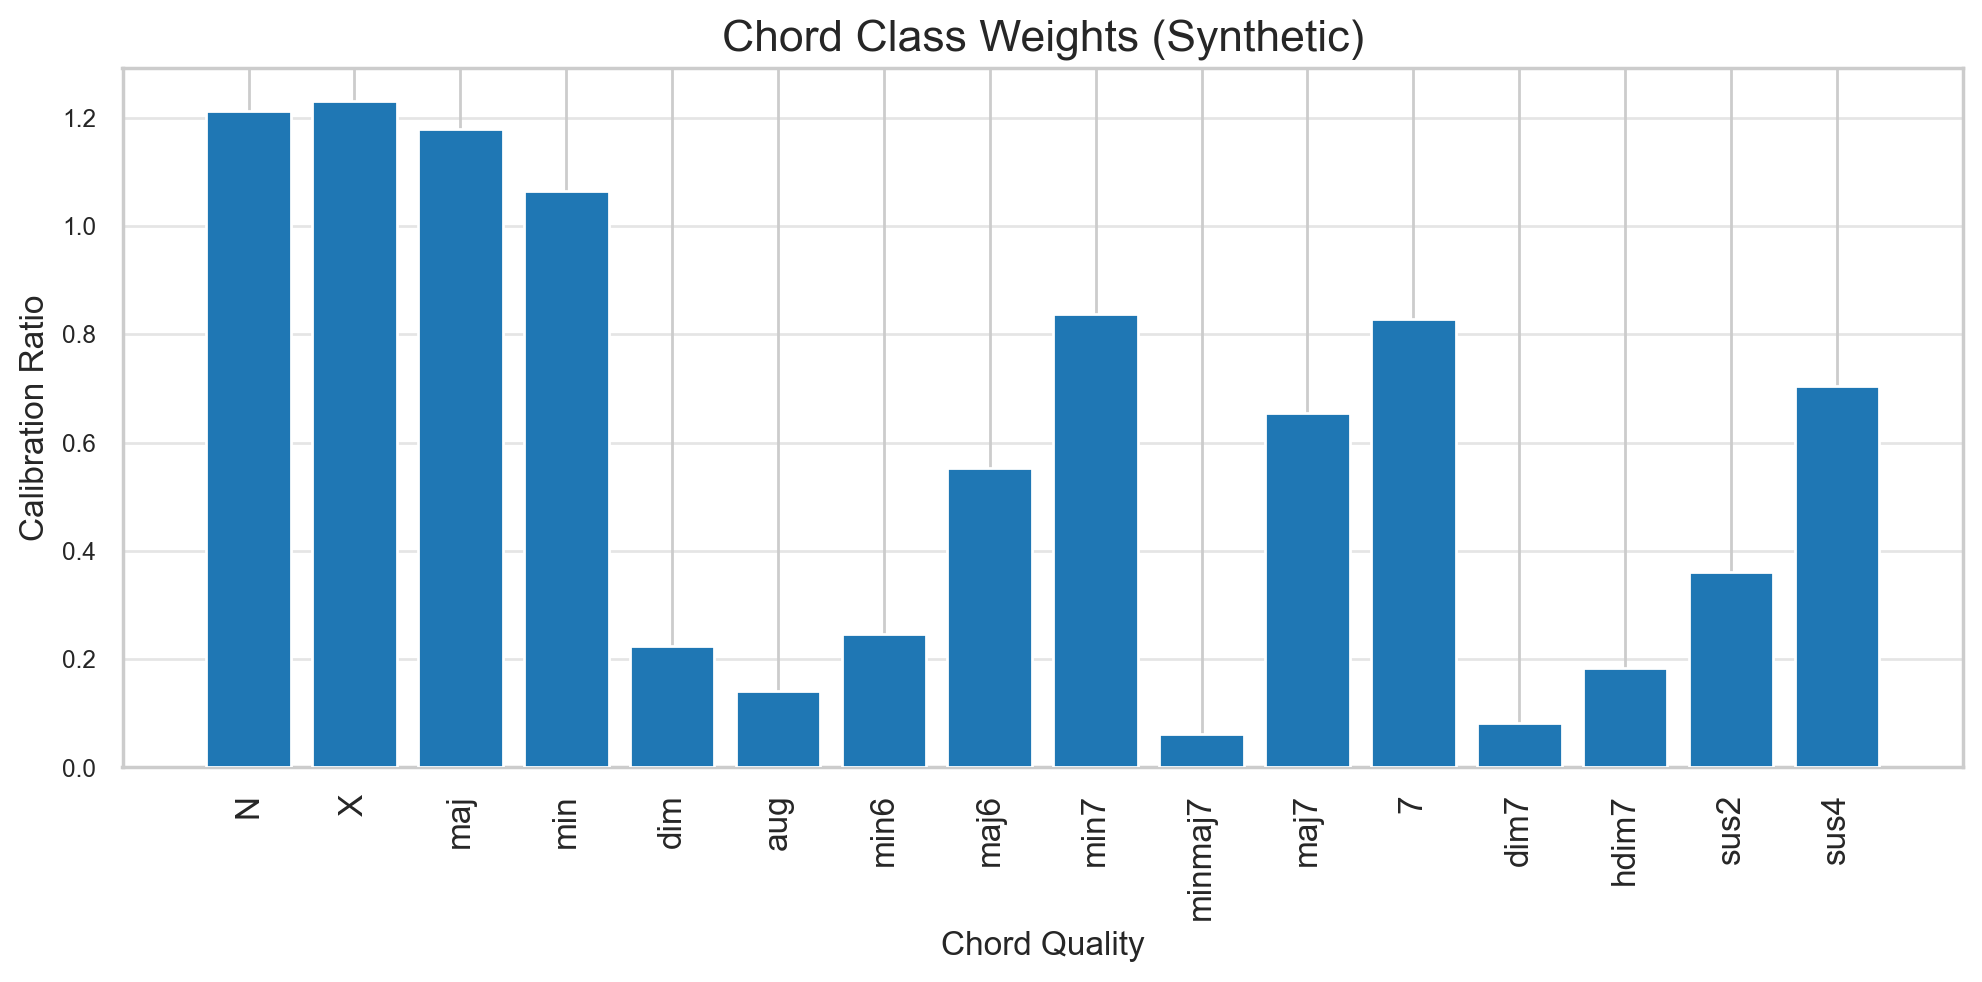
\includegraphics[width=0.8\textwidth]{figures/calibration_ratios.png}
    \caption{Calibration ratios $r_q$ of the model's outputs to account for distribution shift. The high ratio on rare chord qualities like \texttt{majmin} show that these qualities are much more common in the synthetic dta.}\label{fig:calibration}
\end{figure*}

\subsection{Difference in Confusion Matrices with Synthetic Data}\label{app:cm_synthetic_data}

Figure~\ref{fig:cm_synthetic_data} compares the normalised confusion matrices of models trained with and without synthetic data. Incorporating synthetic data reduces predictions of \texttt{X} chords and improves recall for \texttt{min7} and \texttt{dim} qualities, but degrades performance on \texttt{hdim7} and \texttt{min6}. It also shifts certain errors, notably from \texttt{min} to \texttt{maj} in \texttt{7} and \texttt{min7} cases. Despite these changes, overall accuracy remains unchanged, making it unclear which model performs better overall.

\begin{figure*}[h]
    \centering
    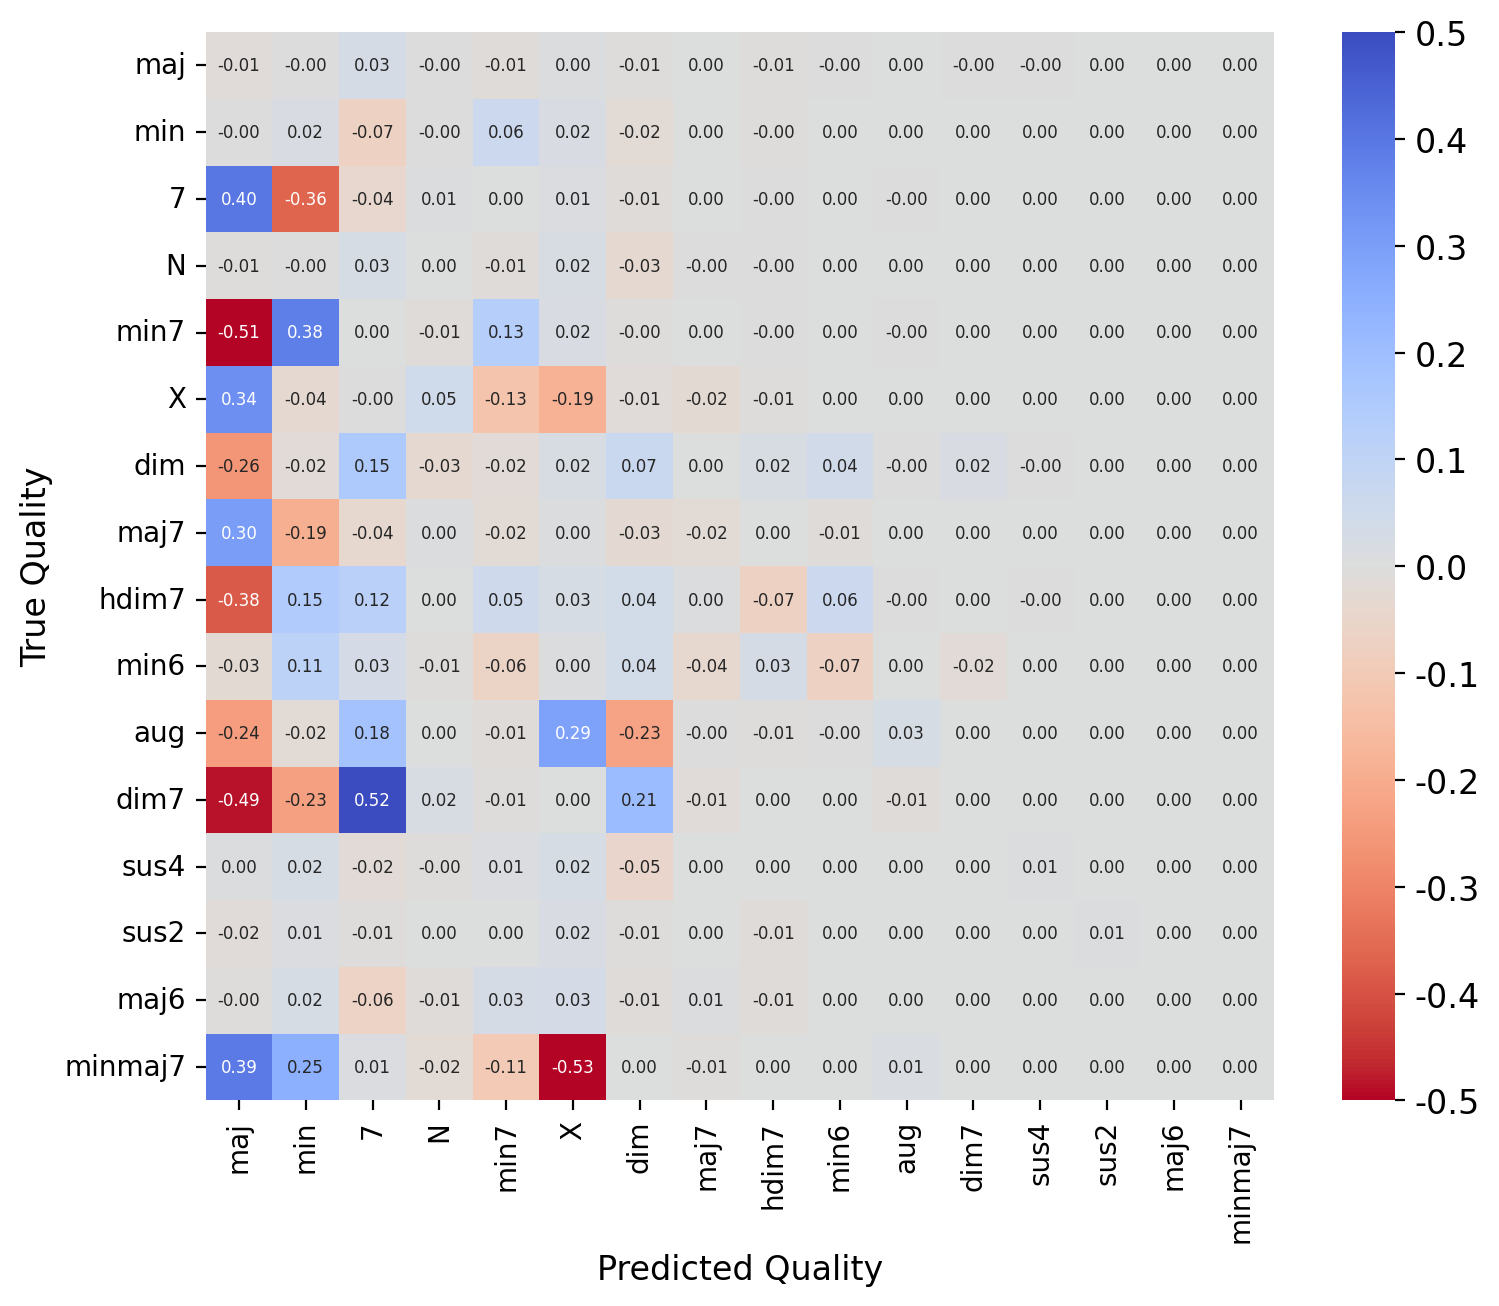
\includegraphics[width=0.8\textwidth]{figures/confusion_matrix_synth.png}
    \caption{Element-wise difference in normalised confusion matrix of the model trained on synthetic data and \emph{pop} data versus just \emph{pop} data with a weighted loss function. There are some notable differences. Training on synthetic data strongly discourages the model from predicting \texttt{X} chords, which are not present in the synthetic data. Recall on \texttt{min7} qualities increases by $13\%$ and by $7\%$ on \texttt{dim} qualities. However, recall \texttt{hdim7} and \texttt{min6} worsens. In general, the model predicts \texttt{maj} less often for rarer qualities. Another interesting observation is that the synthetic data corrects many of the predictions on \texttt{7} qualities from erroneous predictions of \texttt{min} to erroneous predictions of \texttt{maj}. Something similar happens with \texttt{min7} qualities. It is hard to say which model is better. Indeed, their overall accuracies are the same.}\label{fig:cm_synthetic_data}
\end{figure*}